\chapter{Analiza stylu jazdy}

\section{Wstęp}

W rozdziale przedstawiono opis podstawowej funkcjonalności zaprogramowanego urządzenia, stanowiącej analizę stylu jazdy kierowcy. Zawiera on autorskie badania, krótki opis istniejących rozwiązań oraz propozycję własnego algorytmu oceny sposobu jazdy. 

Funkcjonalność opisująca styl jazdy jest niezwykle istotna z punktu widzenia jednej z grup docelowych, do których kierowane jest urządzenie - firm posiadających flotę pojazdów. Wynika to z faktu rosnących kosztów prowadzenia działalności oraz użytkowania pojazdów (w tym wzrostu cen paliwa, części zamiennych i usług). Można do nich zaliczyć nadmiernie szybkie zużycie części eksploatacyjnych, jak na przykład klocków hamulcowych czy opon, a także koszty związane z wypadkami losowymi jak stłuczki. W przypadku firm, są one często generowane przez nieodpowiedzialnych pracowników, którzy nie szanują własności pracodawcy oraz prowadzą pojazdy w sposób lekkmyślny i agresywny. Ograniczenie tego procederu jest o tyle problematyczne, iż trudno o jednoznaczne dowody winy pracownika - kierowcy. Odpowiadając na tę potrzebę rynkową, opisywany w pracy system pozwala nie tylko na ocenę stylu jazdy i jego zdalne monitorowanie na bieżąco, lecz także na zapisywanie historii ocen przypisanych do punktów przebytej przez pracownika trasy wraz z dodatkowymi parametrami, opisywanymi we wcześniejszych rozdziałach. Pozwala to nie tylko na uzyskanie informacji czy pracownik jechał zbyt agresywnie, lecz także kiedy i gdzie to nastąpiło.

\clearpage
\section{Istniejące metody}

W ramach przygotowania do implementacji algorytmu analizy stylu jazdy, dokonano przeglądu artykułów naukowych, opisujących istniejące już metody. Najciekawszy z nich (\cite{driving_analysis_article}) opisuje wykorzystanie telefonu typu smartphone jako platformy czujników pomiarowych. Metoda opisana w artykule jest bardzo podobna do sposobu wykrywania gestów w kontrolerach ruchu dedykowanych do gier.  Wykorzystywane są w tym celu dane z akcelerometru oraz żyroskopu, a także system GPS. Pierwsze dwa z nich umożliwiają wykrycie łagodnych i ostrych skrętów, manewru zawracania, a także przyspieszania i hamowania zarówno gwałtownych, jak i spokojnych. Moduł GPS służy do uzyskania informacji o prędkości pojazdu. Głównym algorytmem wykrywania manewrów jest DTW (\textit{ang. \textbf{D}ynamic \textbf{T}ime \textbf{W}arping}), który służy do wyznaczenia miary podobieństwa pomiędzy dwoma sygnałami. 
Pierwszym krokiem w zastosowaniu algorytmu jest kalibracja telefonu. Autorzy umieszczają telefon na desce rozdzielczej i odpowiednio go orientują względem pojazdu. Działający na nim program dokonuje filtracji danych filtrem dolnoprzepustowym o częstotliwości granicznej 25 Hz ze względu na drgania pochodzące od pracującego silnika. Dane pozyskiwane są w postaci zbioru kilku tysięcy próbek. 
Pierwszym etapem jest wykrycie rozpoczęcia manewru. W tym celu wykorzystano średnią kroczącą:

\begin{equation}
	SMA = \frac{g(i)^2 + g(i-1)^2 + ... + g(i-k-1)^2}{k}
\end{equation}

gdzie
$g(i)$ - wartość próbki przyspieszenia
$k$ - liczba próbek w oknie sygnału

Skok cyklicznie wyliczanej w ten sposób średniej powyżej założonego przez autorów progu traktowany jest jako początek manewru. Trwa on dopóki wartość SMA nie spadnie poniżej progu końca manewru. Jeśli czas trwania wykrytego w ten sposób ruchu jest dłuższy niż 15 sekund, jest on traktowany jako błąd pomiaru i odrzucany.

Wykryte w ten sposób manewry poddawane są następnie przetworzeniu przez algorytm DTW. Pozwala on na znalezienie najmniejszej odległości między dwoma sygnałami, czyli stopnia ich podobieństwa (korelacji). Oznacza to, że w pamięci programu zapisane są pewne uśrednione modele wszystkich wykrywanych manewrów, z którymi porównywane są aktualnie przetwarzane dane. Wyliczona korelacja z modelami jazdy agresywnej może służyć za ocenę stylu jazdy.

Metoda ta pozwala na wykrycie wielu różnych manewrów, lecz jest kosztowna obliczeniowo i pamięciowo. Nie jest to problem dla telefonów będących obecnie na rynku, ale stanowi kluczową kwestię w systemach wbudowanych, posiadających niewielkie zasoby. Ponadto, problemem samego algorytmu jest brak precyzyjnej definicji czym jest manewr łagodny, a czym gwałtowny, przez co bazuje on na subiektywnie wybranych modelach manewrów. Co więcej, fakt zastosowania smartfona powoduje wzrost kosztów systemu, a także konieczność jego cyklicznego ładowania co znacznie utrudnia możliwość jego ukrycia wewnątrz pojazdu.
W związku z faktem, iż praca powstała na Wydziale Mechatroniki, która stanowi interdyscyplinarną, synergiczną dziedzinę łączącą mechanikę, elektronikę i sterowanie, zdecydowano się na przeprowadzenie własnych badań i zaproponowanie autorskiego rozwiązania, które można byłoby zastosować w opisywanym w pracy systemie.

\section{Badania}
\label{experiments}

Na ocenę stylu jazdy kierowcy wpływ mają głównie dwa czynniki - prędkość oraz przyspieszenie. Pierwszy z nich niesie informację jak często i o ile kierowca przekraczał limit dopuszczalny prawem. Wykorzystanie tego parametru jest bardzo proste w implementacji, lecz okazuje się kosztowne. W wykorzystywanej w pracy bibliotece do obsługi map od firmy Google istnieje moduł drogowy (Google Maps Road API\cite{google_map_road_api}), jednak w wersji darmowej (wprowadzającej dzienne limity zapytań) nie jest udostępniona informacja o ograniczeniach prędkości na drogach. Aby z niej skorzystać należy wykupić licencję Premium. Z tego powodu postanowiono zrezygnować z czynnika przekraczania prędkości w zautomatyzowanej analizie, a wartość bezwzględną szybkości pozostawić do oceny indywidualnej.

Drugim, znacznie ciekawszym parametrem jest przyspieszenie. Jest ono tak interesujące, ponieważ ma wpływ nie tylko na bezpieczeństwo, lecz także na ponoszone przez pracodawcę koszty. Znaczne przyspieszenie powoduje:

\begin{itemize}
\item Zużycie opon w przypadku zerwania przyczepności przy ruszaniu
\item Oderwanie odważników wyważających koła co nie tylko wpływa na komfort jazdy, lecz również na elementy zawieszenia pojazdu (drgania)
\item Zużycie sprzęgła w przypadku agresywnego ruszania
\item Duże obciążenie elementów przeniesienia napędu
\item Szybsze zużycie elementów wewnętrznych silnika
\item Wysokie zużycie paliwa i wzrost zanieczyszczeń wydzielanych do atmosfery
\item Zużycie klocków, przegrzanie i wygięcie tarcz hamulcowych w przypadku gwałtownego hamowania
\item Możliwość wejścia w poślizg i utraty kontroli nad pojazdem co może skutkować uderzeniem w barierki lub inne pojazdy
\end{itemize}

Dodatkowo, w ramach rozważań uwzględniono, że wpływ na bezpieczeństwo i ekonomię ma nie tylko wartość akceleracji, lecz także jego zmienność reprezentowana przez zryw, czyli pochodną przyspieszenia po czasie. Z tego powodu postanowiono wykorzystać zamontowany na płytce lokalizatora akcelerometr i zbadać przebiegi przyspieszenia oraz zrywu w osiach X, Y i Z w trakcie wykonywania różnych manewrów na drodze. W każdym z testów poczyniono założenie o odpowiedniej orientacji urządzenia względem pojazdu. Zostało ono w każdym przypadku ustawione tak, aby oś Y pokrywała się z kierunkiem jazdy na wprost, oś Z była umieszczona prostopadle do podłoża, a wynikowo oś X wskazywała kierunek od drzwi do drzwi pojazdu.

W trakcie eksperymentów bardzo istotne było wyeliminowanie wpływu przyspieszenia ziemskiego oraz jego rzutów na osie X i Y, wynikających z niedokładnej orientacji urządzenia. W związku z tym, po uruchomieniu, przez sekundę zbiera ono próbki przyspieszeń, po czym dokonuje ich uśrednienia i zapisuje wyniki w pamięci. Zmierzone w ten sposób wartości są odejmowane od każdej pobranej z akcelerometru próbki. Dzięki zastosowaniu tej metody uzyskano bardzo dokładną kompensację wpływu grawitacji przy braku ruchu pojazdu. Końcowy wynik pomiaru w tym przypadku był rzędu 0.005 $\frac{m}{s^2}$.

Testy rozpoczęto od najniższej dostępnej częstotliwości próbkowania - 12.5 Hz, w celu osiągnięcia jak najmniejszego zużycia energii przez akcelerometr i ograniczenia liczby niezbędnych do wykonania działań. Wyniki przedstawiono na rysunku \ref{fig:image_driving_analysis_test_12Hz}. W przypadku tego testu, ujemna część osi Y skierowana była zgodnie z ruchem pojazdu, oś X wskazywała przyspieszenia boczne, a oś Z - przyspieszenia pionowe.

\begin{figure}[H]
	\centering
	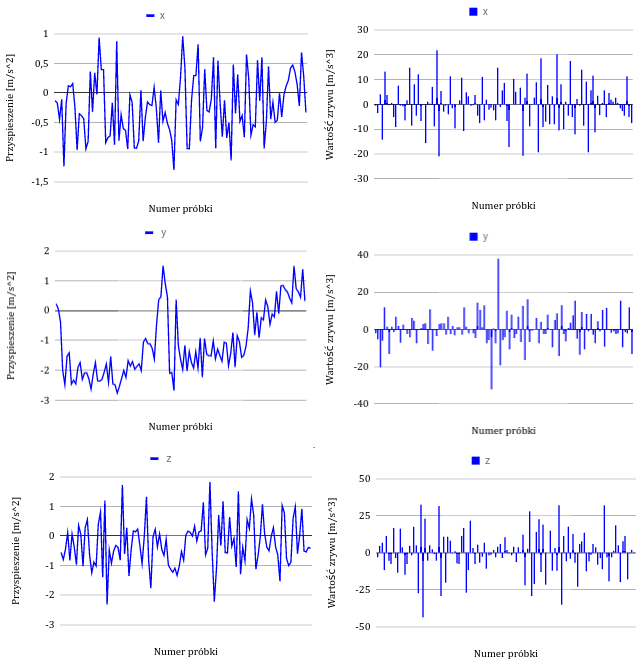
\includegraphics[width=12cm]{img/driving_analysis/12_5Hz_Przyspieszanie.png}
	\caption{Wykresy przyspieszenia i zrywu w trakcie przyspieszania przy częstotliwości próbkowania 12.5 Hz.
	\\Źródło: Opracowanie własne.}
	\label{fig:image_driving_analysis_test_12Hz}
\end{figure}

Jak widać, dane (zwłaszcza te dotyczące zrywu) wydają się niekompletne, "poszatkowane". W wyniku obserwacji wyników pierwszych testów postanowiono zrezygnować z uwzględniania przyspieszeń w osi Z ze względu na ich znikomy wkład w opis stylu jazdy kierowcy.

Następnym krokiem badań było sprawdzenie wpływu zwiększenia częstotliwości próbkowania o jeden krok - do 26 Hz. W przypadku tego testu skorygowano pomyłkę orientacji urządzenia tak, aby zwrot osi Y pokrywał się z kierunkiem jazdy na wprost. Pozostałe warunki orientacji pozostały bez zmian. Wyniki badań przedstawiono na rysunkach \ref{fig:image_driving_analysis_test_26Hz} i \ref{fig:image_driving_analysis_test_acc_26Hz}.

\begin{figure}[H]
	\centering
	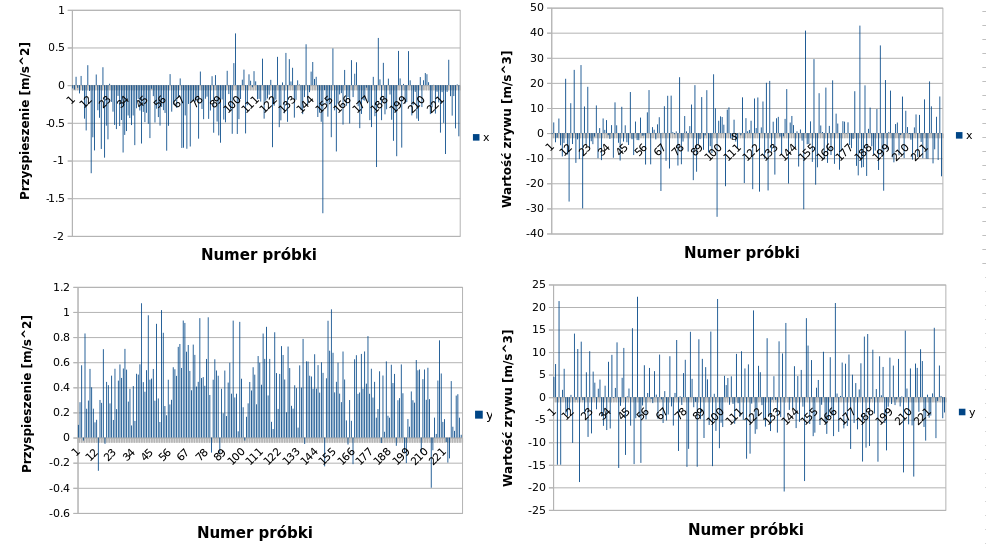
\includegraphics[width=15cm]{img/driving_analysis/stabilna_26.png}
	\caption{Wykresy przyspieszenia i zrywu w trakcie stabilnej jazdy przy częstotliwości próbkowania 26 Hz.
	\\Źródło: Opracowanie własne.}
	\label{fig:image_driving_analysis_test_26Hz}
\end{figure}

\begin{figure}[H]
	\centering
	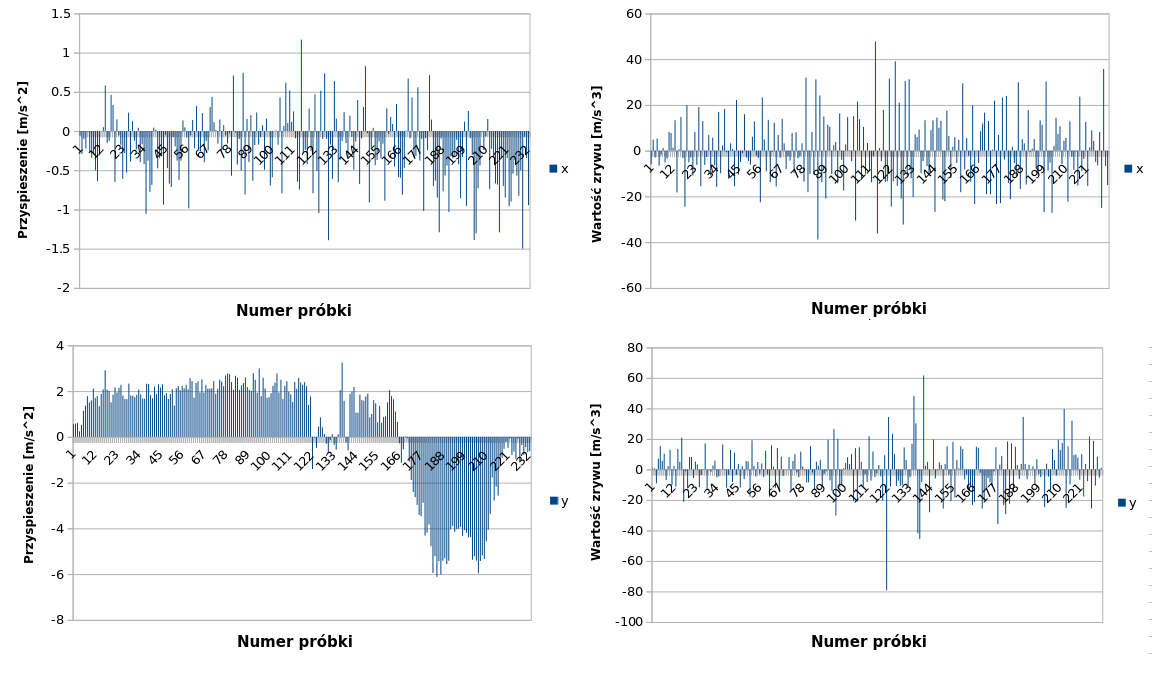
\includegraphics[width=15cm]{img/driving_analysis/Ostre_przyspieszenie_26Hz.png}
	\caption{Wykresy przyspieszenia i zrywu w trakcie agresywnego przyspieszania i hamowania przy częstotliwości próbkowania 26 Hz.
	\\Źródło: Opracowanie własne.}
	\label{fig:image_driving_analysis_test_acc_26Hz}
\end{figure}

\clearpage
Jak widać, wzrost częstotliwości bardzo pozytywnie wpłynął na jakość zebranych danych w przypadku przyspieszenia, lecz wyznaczone wartości zrywu wciąż wydają się niekompletne. Kolejnym wnioskiem pochodzącym z obserwacji jest fakt, iż dla agresywnego przyspieszania i hamowania występują różne zakresy osiąganych wartości przyspieszeń. Jest to wynik spodziewany, gdyż zazwyczaj zdolność pojazdów do hamowania jest znacznie większa niż do przyspieszania. 

Po zebraniu kilku innych zestawów próbek, postanowiono dokonać dalszego zwiększenia częstotliwości próbkowania o kolejny krok - do 52 Hz. Wyniki dla jazdy na wprost ze stałą prędkością przedstawiono na rysunku \ref{fig:image_driving_analysis_test_52Hz}.

\begin{figure}[H]
	\centering
	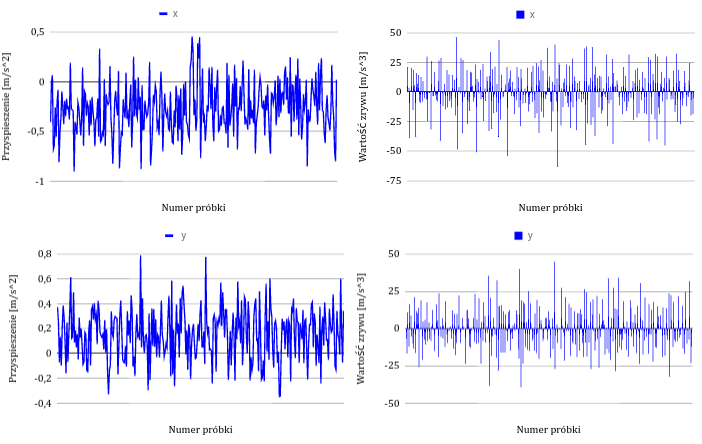
\includegraphics[width=15cm]{img/driving_analysis/stabilna_52.png}
	\caption{Wykresy przyspieszenia i zrywu w trakcie stabilnej jazdy przy częstotliwości próbkowania 52 Hz.
	\\Źródło: Opracowanie własne.}
	\label{fig:image_driving_analysis_test_52Hz}
\end{figure}

Na powyższym obrazku widać, że dane są już kompletne, nie wykazują nagłej zmienności. Z tego powodu zdecydowano się na zastosowanie w urządzeniu częstotliwości próbkowania wynoszącej 52 Hz. Częstotliwość ta stanowi dodatkowo kompromis pomiędzy dokładnością danych, a czasem ich przetwarzania i niezbędną ilością pamięci w mikrokontrolerze do ich zgromadzenia. Pozostałe przypadki rozpatrywanych zachowań na drodze przedstawiono na rysunkach: \ref{fig:image_driving_analysis_test_acc_light_aggressive_52Hz} i \ref{fig:image_driving_analysis_test_acc_light_hard_lane_52Hz}.

\begin{figure}[H]
	\centering
	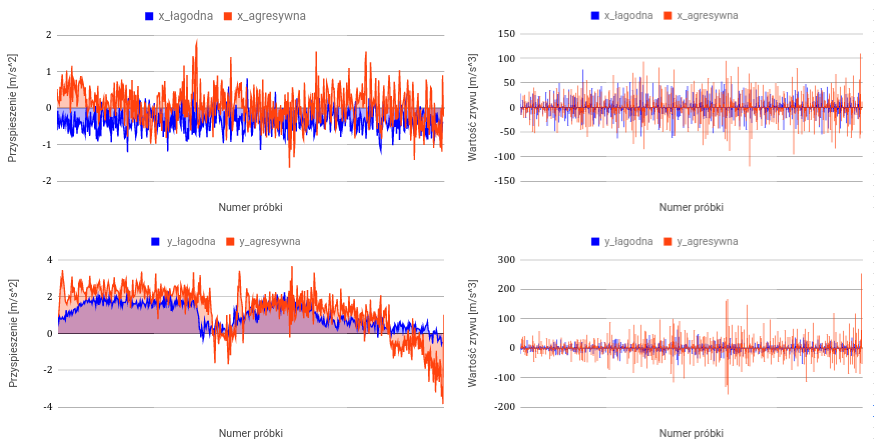
\includegraphics[width=16cm]{img/driving_analysis/zestawienie_lagodna_ostra-ruszanie.png}
	\caption{Zestawienie wykresów przyspieszenia i zrywu w trakcie łagodnego i agresywnego ruszania przy częstotliwości próbkowania 52 Hz.
	\\Źródło: Opracowanie własne.}
	\label{fig:image_driving_analysis_test_acc_light_aggressive_52Hz}
\end{figure}

\begin{figure}[H]
	\centering
	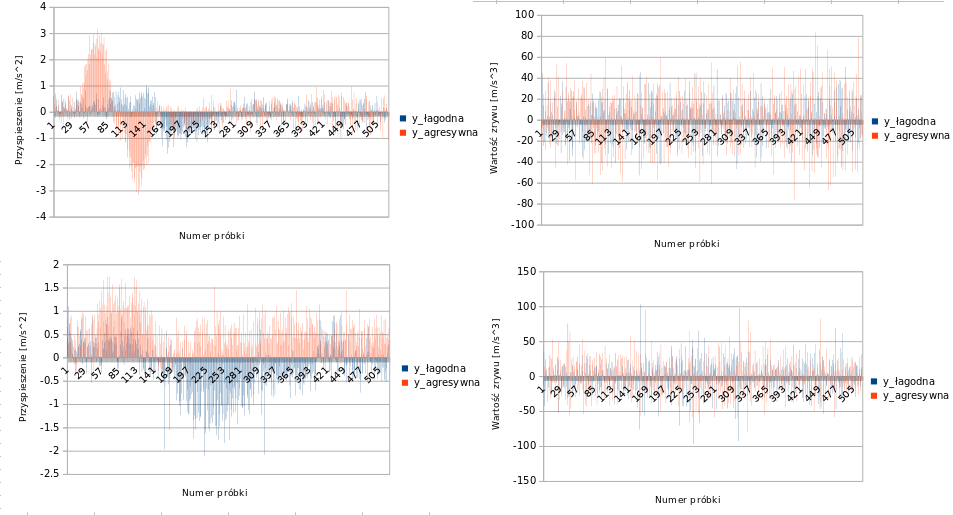
\includegraphics[width=16cm]{img/driving_analysis/zestawienie_ostra_lagodna.png}
	\caption{Zestawienie wykresów przyspieszenia i zrywu w trakcie łągodnej i agresywnej zmiany pasa przy częstotliwości próbkowania 52 Hz.
	\\Źródło: Opracowanie własne.}
	\label{fig:image_driving_analysis_test_acc_light_hard_lane_52Hz}
\end{figure}

Obserwując powyższe wykresy można zauważyć, że są one na tyle dokładne, iż widać na nich nawet moment zmiany biegu (nagły, krótkotrwały spadek przyspieszenia dla osi Y). Można również dostrzec, że wartości przyspieszeń w przypadku łagodnego i agresywnego przyspieszania nie różnią się od siebie znacząco, w przeciwieństwie do ich chwilowych zmian, opisywanych przez zryw. Jest to rezultat rozbieżności stopni przełożeń w skrzyni biegów, które są tak dobrane, aby pojazd uzyskiwał większe przyspieszenie na niskich biegach niż na wysokich. W efekcie oznacza to, że wartość przyspieszenia nie może stanowić głównego czynnika oceny stylu jazdy.

Kolejnym wnioskiem na podstawie obserwacji uzyskanych danych jest fakt, iż w przypadku łagodnej zmiany pasa pojazd zwalniał (ujemne przyspieszenie w osi Y), a w przypadku agresywnej - przyspieszał (dodatnie przyspieszenie w osi Y). Informacja ta jest bardzo ciekawa, gdyż wskazuje na dodatkową korelację pomiędzy stylem jazdy w osiach X i Y przy zmianie pasa ruchu, co powoduje wzmocnienie jego negatywnej lub pozytywnej oceny.

W celu poprawienia widoczności zależności opisującej styl jazdy w danych dotyczących zrywów, parametry te zestawiono na histogramach przedstawionych na rysunkach \ref{fig:image_histogram_acceleration_52Hz} i \ref{fig:image_histogram_changing_lane_52Hz}.

\begin{figure}[H]
	\centering
	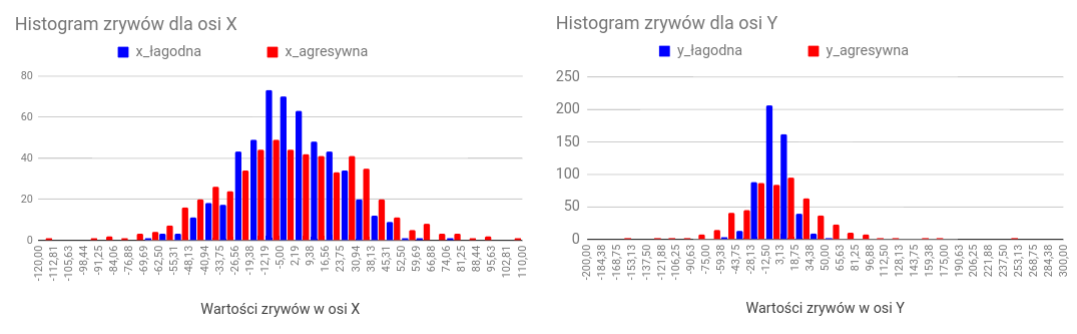
\includegraphics[width=16cm]{img/driving_analysis/histogram_zestawienie_ostre_lagodne_ruszanie.png}
	\caption{Zestawienie histogramów zrywu w osiach X i Y w trakcie łagodnego i agresywnego ruszania przy częstotliwości próbkowania 52 Hz.
	\\Źródło: Opracowanie własne.}
	\label{fig:image_histogram_acceleration_52Hz}
\end{figure}

\begin{figure}[H]
	\centering
	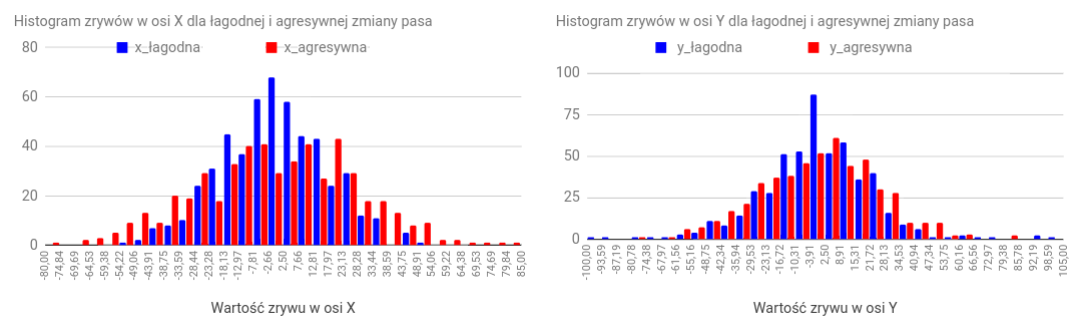
\includegraphics[width=16cm]{img/driving_analysis/histogram_zestawienie_zmiana_pasa.png}
	\caption{Zestawienie histogramów zrywu w osiach X i Y w trakcie łagodnej i agresywnej zmiany pasa przy częstotliwości próbkowania 52 Hz.
	\\Źródło: Opracowanie własne.}
	\label{fig:image_histogram_changing_lane_52Hz}
\end{figure}

Jak widać, w przypadku jazdy agresywnej, histogramy opisujące ruch w osi głównej (dla zmiany pasa ruchu - oś X, dla jazdy na wprost - oś Y) ulegają spłaszczeniu i rozszerzeniu. Oznacza to, że mniej próbek uzyskuje niską wartość bezwzględną zrywu, a więcej wysoką, w porówaniu do histogramu dla jazdy łagodnej. Stanowi to potwierdzenie tezy o wzroście wariancji pochodnej przyspieszenia wraz ze wzrostem poziomu agresji stylu jazdy.

Podsumowując, na podstawie danych przedstawionych na powyższych rysunkach otrzymano następujące wnioski:

\begin{itemize}
\item Dane nie posiadają znaczącego czynnika losowego w postaci szumu, zatem nie jest konieczne ich dodatkowe filtrowanie.
\item Wartość i rozkład przyspieszenia w obrębie okna czasowego, w czasie którego gromadzono próbki bardzo wyraźnie informują o rodzaju wykonywanego manewru.
\item Wartość zrywu jest w przybliżeniu symetryczna względem zera. Oznacza to, że jego średnia wartość w całym zakresie próbek jest bardzo niewielka.
\item Wraz ze wzrostem poziomu agresji stylu jazdy, wartość wariancji zrywu oraz moduł przyspieszenia średniego rośnie, przy czym pierwszy parametr wykazuje większą zmienność w zależności od sposobu jazdy. 
\end{itemize}

\section{Metoda zastosowana w pracy}

Metoda powstała na podstawie analizy wniosków z podrozdziału \ref{experiments}. W swych podstawach wykorzystuje ona przyspieszenie oraz wariancję zrywu. Jedynym jej założeniem jest konieczność odpowiedniej orientacji urządzenia względem kierunku jazdy. Mianowicie, jak już zostało wcześniej wspomniane, oś Y akcelerometru musi pokrywać się z kierunkiem jazdy na wprost, a oś Z powinna być skierowana prostopadle do podłoża. Algorytm jest następujący:

\begin{enumerate}
\item Pobierz wartości przyspieszeń zgromadzone w pamięci akcelerometru z okresu pomiędzy próbkami lokalizacji (domyślnie 10 sekund).
\item Dla otrzymanego zbioru danych wylicz wartości zrywu dla osi X i Y.
\item Podziel zbiór próbek na okna czasowe o szerokości 0.5 sekundy. Zastosowanie tego kroku pozwala na kwantyzację czasową w celu uśrednienia danych. Szerokość okna została dobrana na podstawie wyników badań z podrozdziału \ref{experiments} tak, aby w wyniku uśredniania nie utracić informacji o krótkotrwałych skokach wartości.
\item Dla każdego okna wylicz przyspieszenia średnie w osiach X i Y, a także wariancję zrywów w tych osiach.
\item Normalizuj każdy z powyższych parametrów, dzieląc go przez pewien dobrany eksperymentalnie próg ustalony dla danej osi, wyróżniając przy tym przyspieszanie od hamowania w kierunku jazdy na wprost, ze względu na konieczność zastosowania odrębnych progów normalizujących.
\item Od każdego ze znormalizowanych parametrów odejmij wartość stałą stanowiącą jego odpowiednik dla jazdy z jednostajną prędkością. Krok ten jest efektem rozumowania, iż agresywny styl jazdy jest niejako stylem łagodnym, z nałożonym na niego pewnym wzorcem ostrej jazdy. Dzięki niemu, oceniany jest jedynie zmienny wpływ czynnika "agresywności", bez uwzględniania wpływu od jazdy ze stałą prędkością.
\item Oblicz ocenę złożoną dla każdej z osi X i Y. Stanowi ona średnią ważoną składowych średniego przyspieszenia znormalizowanego i znormalizowanej wariancji zrywu z wagami wynoszącymi odpowiednio 1 i 2. Wynika to z faktu, iż na podstawie obserwacji danych przedstawionych w podrozdziale \ref{experiments}, wariancja zrywu wykazuje lepszą zdolność do klasyfikacji sposobu jazdy.
\item Wyznaczenie oceny dla próbki jako średniej arytmetycznej ocen z osi X i Y.
\item Wyznaczenie oceny całej trasy jako średniej ważonej ocen każdej próbki należącej do tej trasy. Oceny powyżej progu 50\% posiadają wagę 1, natomiast te poniżej tej wartości - 2. Ma to na celu wzmocnienie reakcji algorytmu w przypadku agresywnej jazdy tak, aby ocena trasy ulegała bardziej zdecydowanie obniżeniu w przypadku zbyt dynamicznego sposobu jazdy.
\end{enumerate}

Algorytm ten przedstawiono na rysunku \ref{fig:image_driving_analysis_alghoritm}.

\begin{figure}[H]
	\centering
	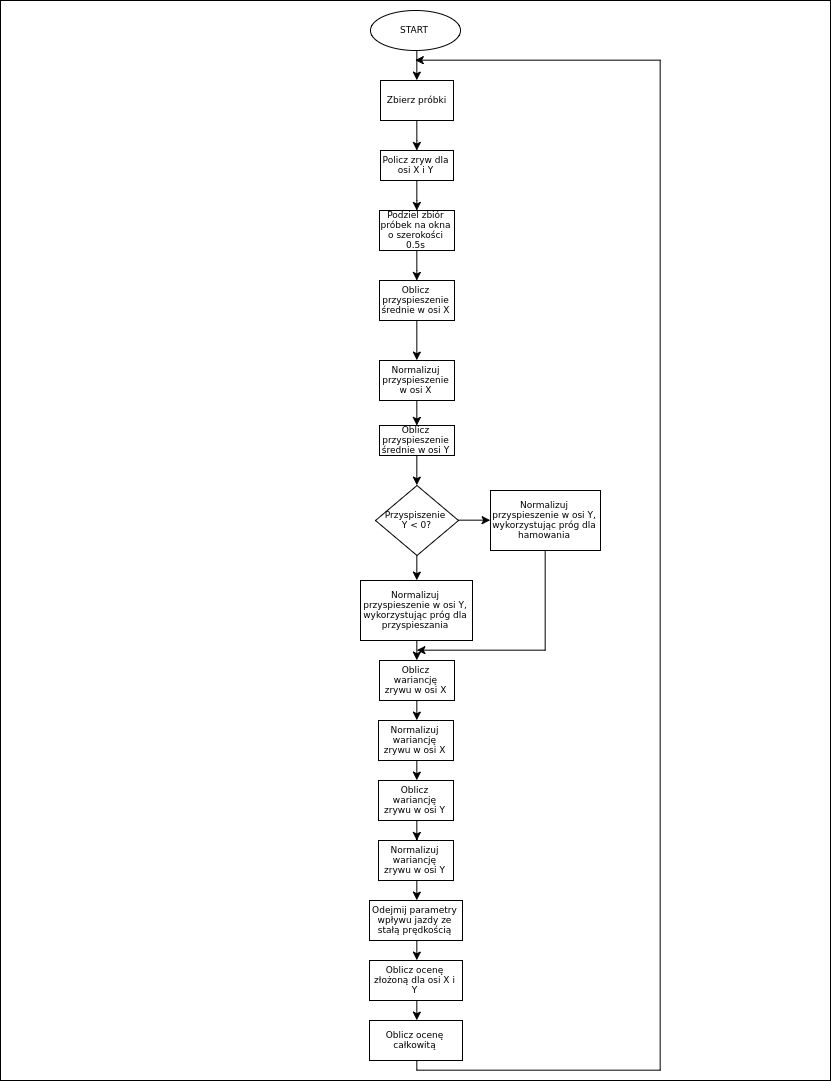
\includegraphics[width=15cm]{img/driving_analysis/driving_analysis.png}
	\caption{Algorytm oceny stylu jazdy. Źródło: Opracowanie własne.}
	\label{fig:image_driving_analysis_alghoritm}
\end{figure}

Wyliczona ocena zawiera się w przedziale $[0.00; 1,00]$, gdzie wynik 0.00 oznacza jazdę łagodną, a 1.00 - bardzo agresywną. Na stronie internetowej są one przedstawiane w skali procentowej, gdzie 0\% oznacza bardzo agresywną jazdę, a 100\% bardzo spokojną. Ponadto, są one wizualizowane na kolorowym pasku, którego barwa płynnie określa ocenę stylu jazdy.

\section{Rezultaty}

W ramach dokonywania testów skuteczności algorytmu, wykonano kilka przejazdów samochodem po różnych trasach. Jedną z wielu tras przedstawiono na rysunku \ref{fig:image_driving_analysis_alghoritm_track_1}.

\begin{figure}[H]
	\centering
	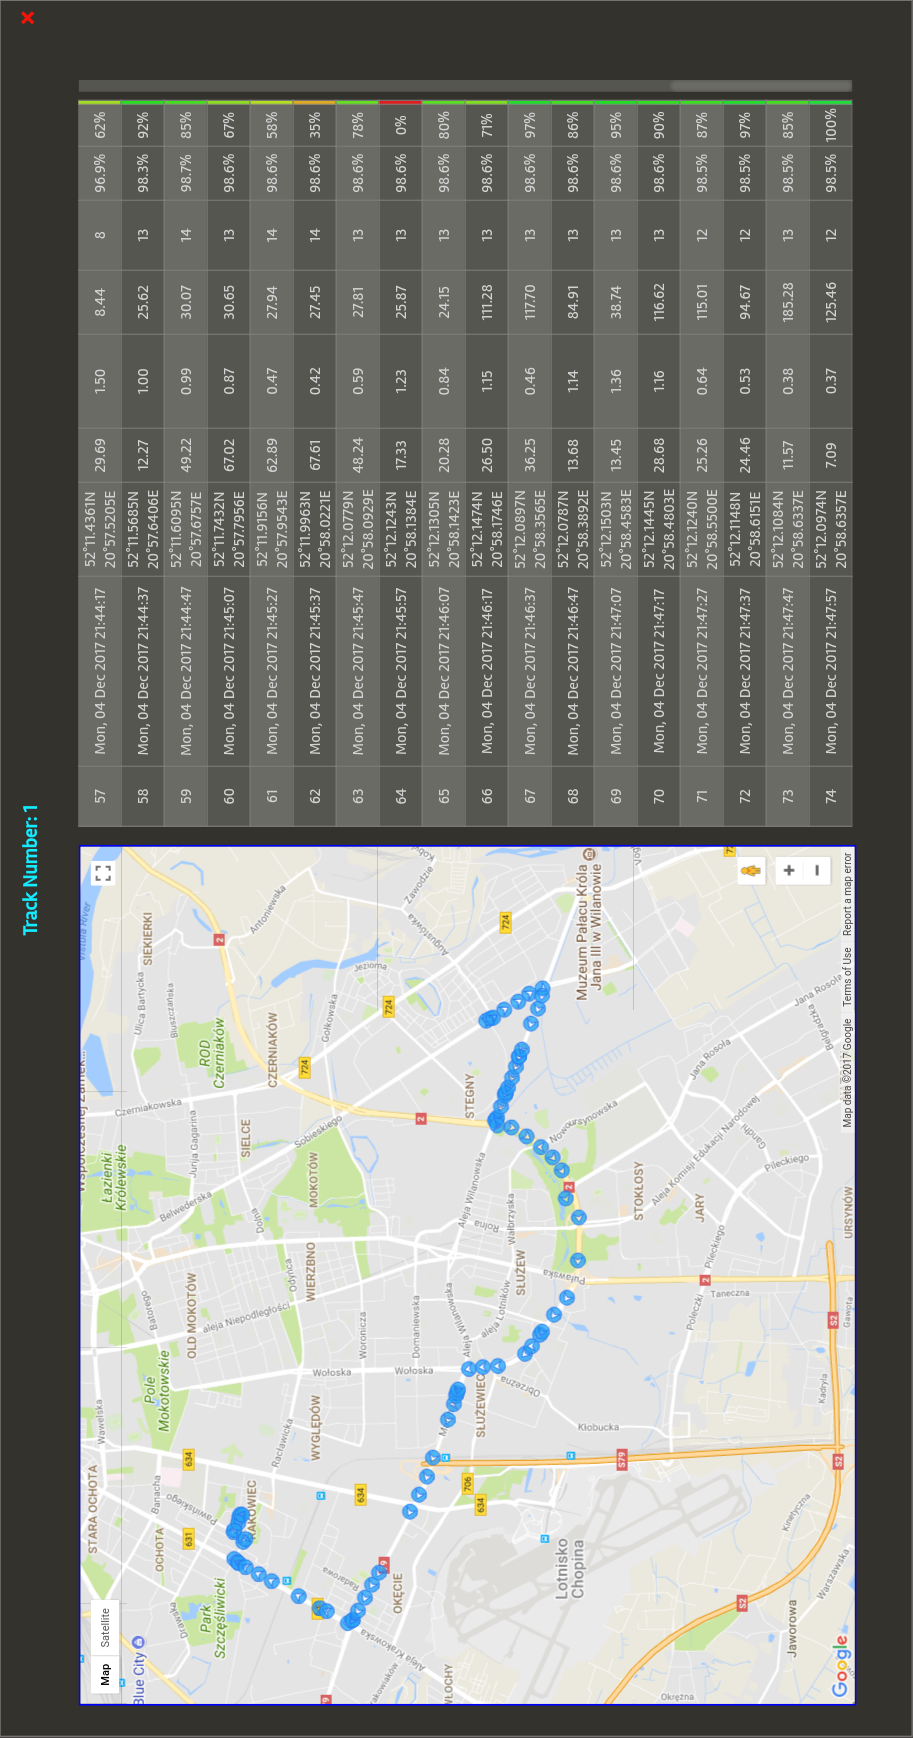
\includegraphics[height=19cm, width=13cm]{img/driving_analysis/test_track_1.png}
	\caption{Trasa próbna nr 1. Źródło: Opracowanie własne.}
	\label{fig:image_driving_analysis_alghoritm_track_1}
\end{figure}

Start nastąpił o godzinie 21:30:59 z ulicy Sobieskiego w Warszawie. Poruszano się w kierunku Wilanowa, a następnie dokonano skrętu w ul. Wilanowską w kierunku zachodnim aż do skrzyżowania z Doliną Służewiecką. Przejazd do tego momentu był łagodny, bez ostrych zmian pasów czy przyspieszeń. Wyniki przedstawiono na rysunku \ref{fig:image_driving_analysis_alghoritm_track_1_part_1}.

\begin{figure}[H]
	\centering
	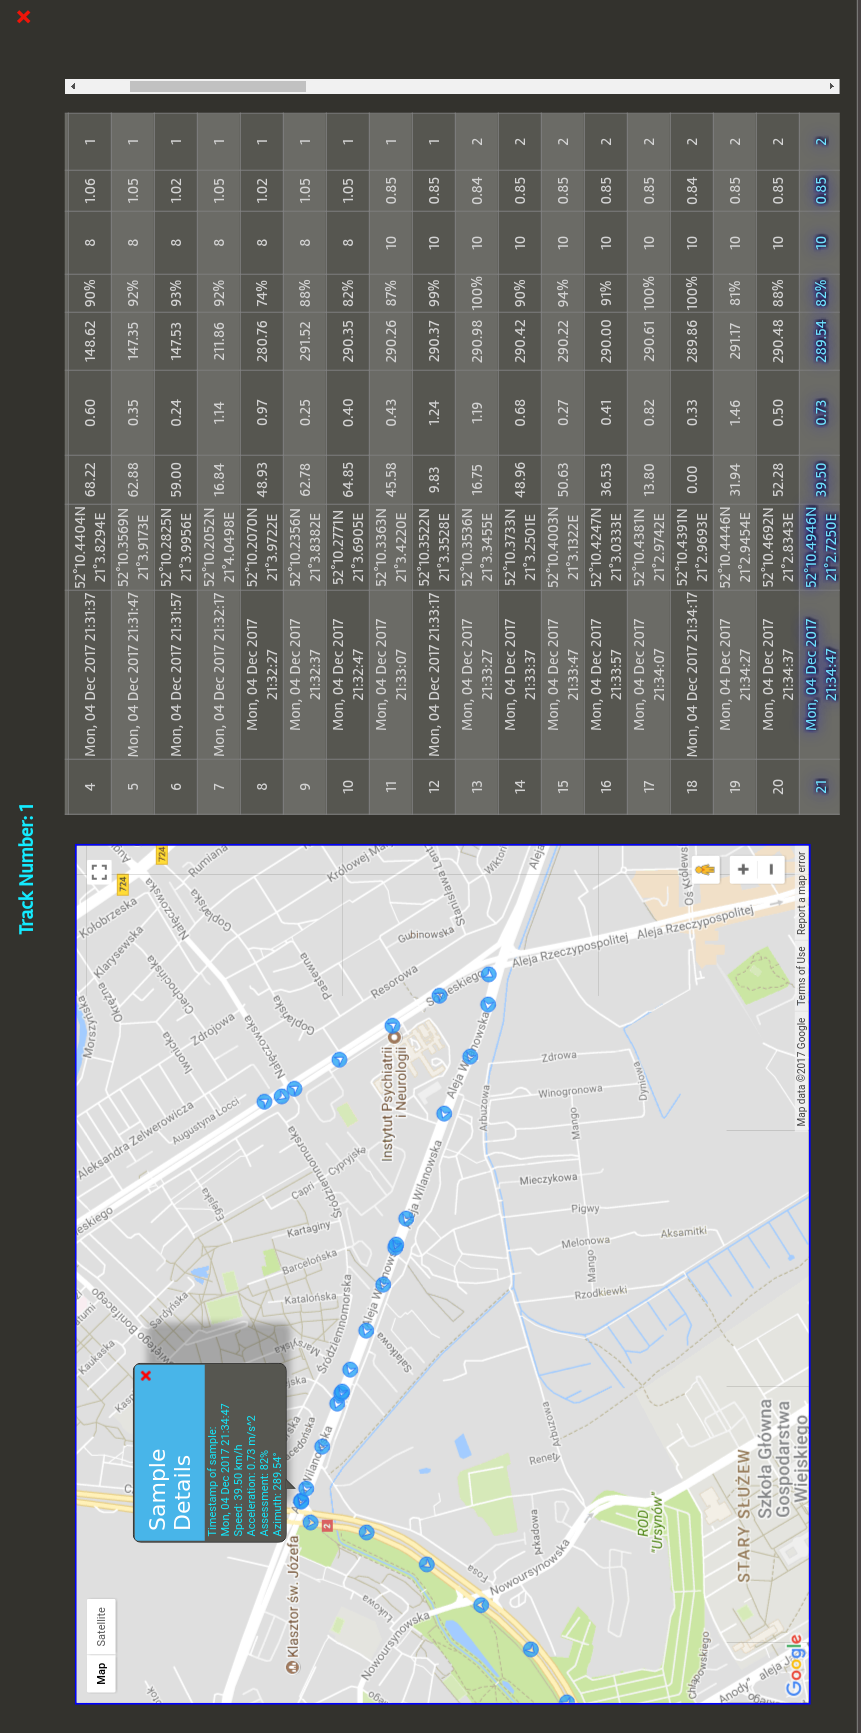
\includegraphics[height=19cm, width=13cm]{img/driving_analysis/test_track_1_lagodna.png}
	\caption{Trasa próbna nr 1 - pierwsza częśś trasy. Źródło: Opracowanie własne.}
	\label{fig:image_driving_analysis_alghoritm_track_1_part_1}
\end{figure}

Następnie skręcono w Dolinę Slużewiecką, przechodzącą w ulicę Rzymowskiego i poruszano się nią aż do skrzyżowania z ulicą Marynarską. Krótko po rozpoczęciu poruszania się Doliną Służewiecką dokonano zwiększenia dynamiki jazdy - bardziej zdecydowanie przyspieszano oraz kilkukrotnie zmieniano pasy ruchu. Manerwy te jednak nie były w stopniu, który można by określić agresywnym, bądź niebezpiecznym. Przedstawiono to na rysunku \ref{fig:image_driving_analysis_alghoritm_track_1_part_2}.

\begin{figure}[H]
	\centering
	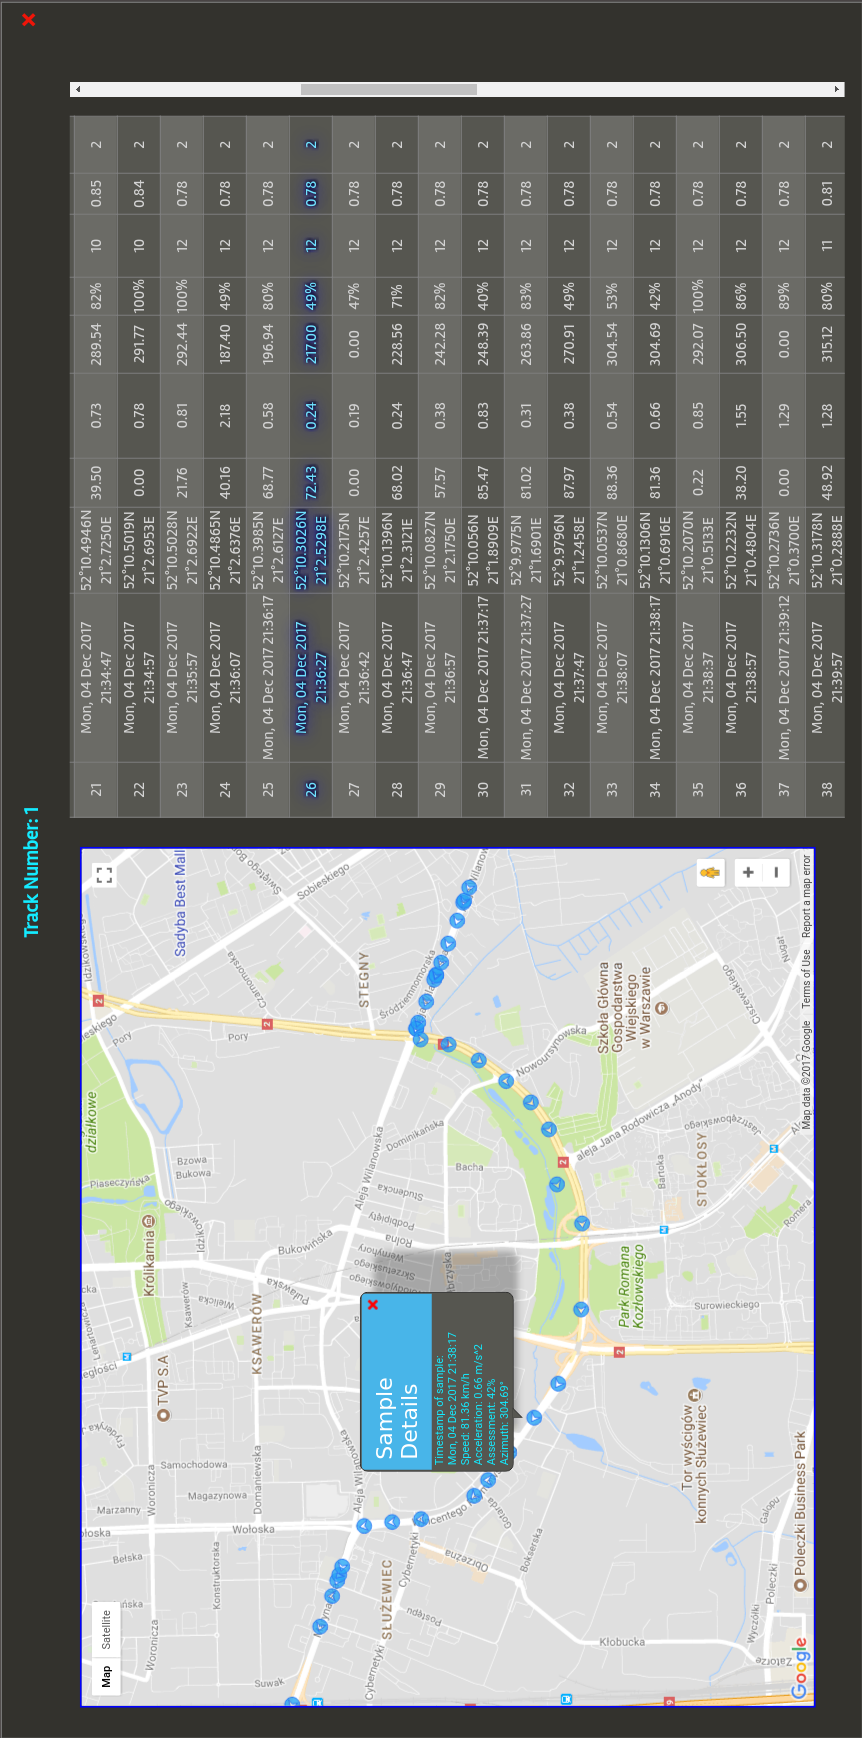
\includegraphics[height=19cm, width=13cm]{img/driving_analysis/test_track_part_2.png}
	\caption{Trasa próbna nr 1 - druga część trasy. Źródło: Opracowanie własne.}
	\label{fig:image_driving_analysis_alghoritm_track_1_part_2}
\end{figure}

Kolejnym etapem był wjazd w ulicę Marynarską i jazda nią aż do Alei Krakowskiej. Od pewnego momentu pierwszej z nich, mniej więcej na wysokości trasy S79 występuje podwyższenie dopuszczalnej prędkości do 80 km/h. Tam dokonano testów agresywnej jazdy. Polegały one na cyklicznym, chwilowym, lecz częstym, mocnym przyspieszaniu oraz gdy warunki na to pozwalały - hamowaniu. Ostre hamowanie nastąpiło tuż przed zjazdem w ulicę Aleja Krakowska. Wyniki testów przedstawiono na rysunku \ref{fig:image_driving_analysis_alghoritm_track_1_part_3}.

\begin{figure}[H]
	\centering
	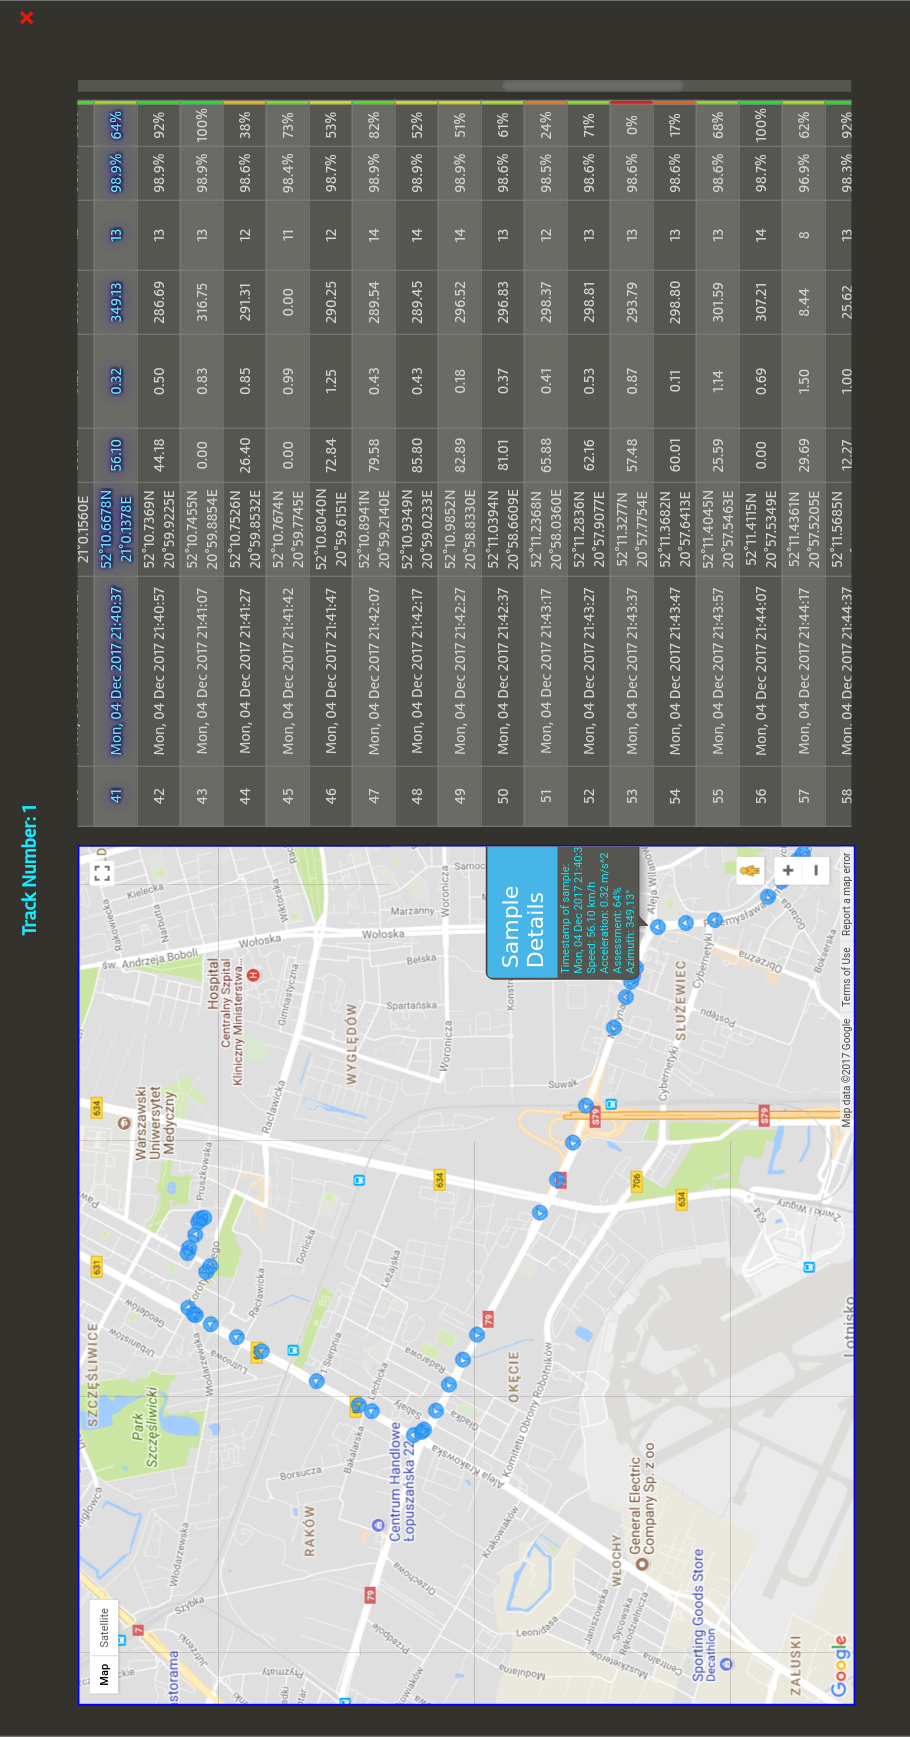
\includegraphics[height=18cm, width=13cm]{img/driving_analysis/test_track_part_3.png}
	\caption{Trasa próbna nr 1 - trzecia część trasy. Źródło: Opracowanie własne.}
	\label{fig:image_driving_analysis_alghoritm_track_1_part_3}
\end{figure}

Ostatnia część trasy - przejazd ulicami: Aleja Krakowska, Korotyńskiego i Pruszkowska przebiegł już łagodnie, co przedstawiono na rysunku \ref{fig:image_driving_analysis_alghoritm_track_1_part_4}.

\begin{figure}[H]
	\centering
	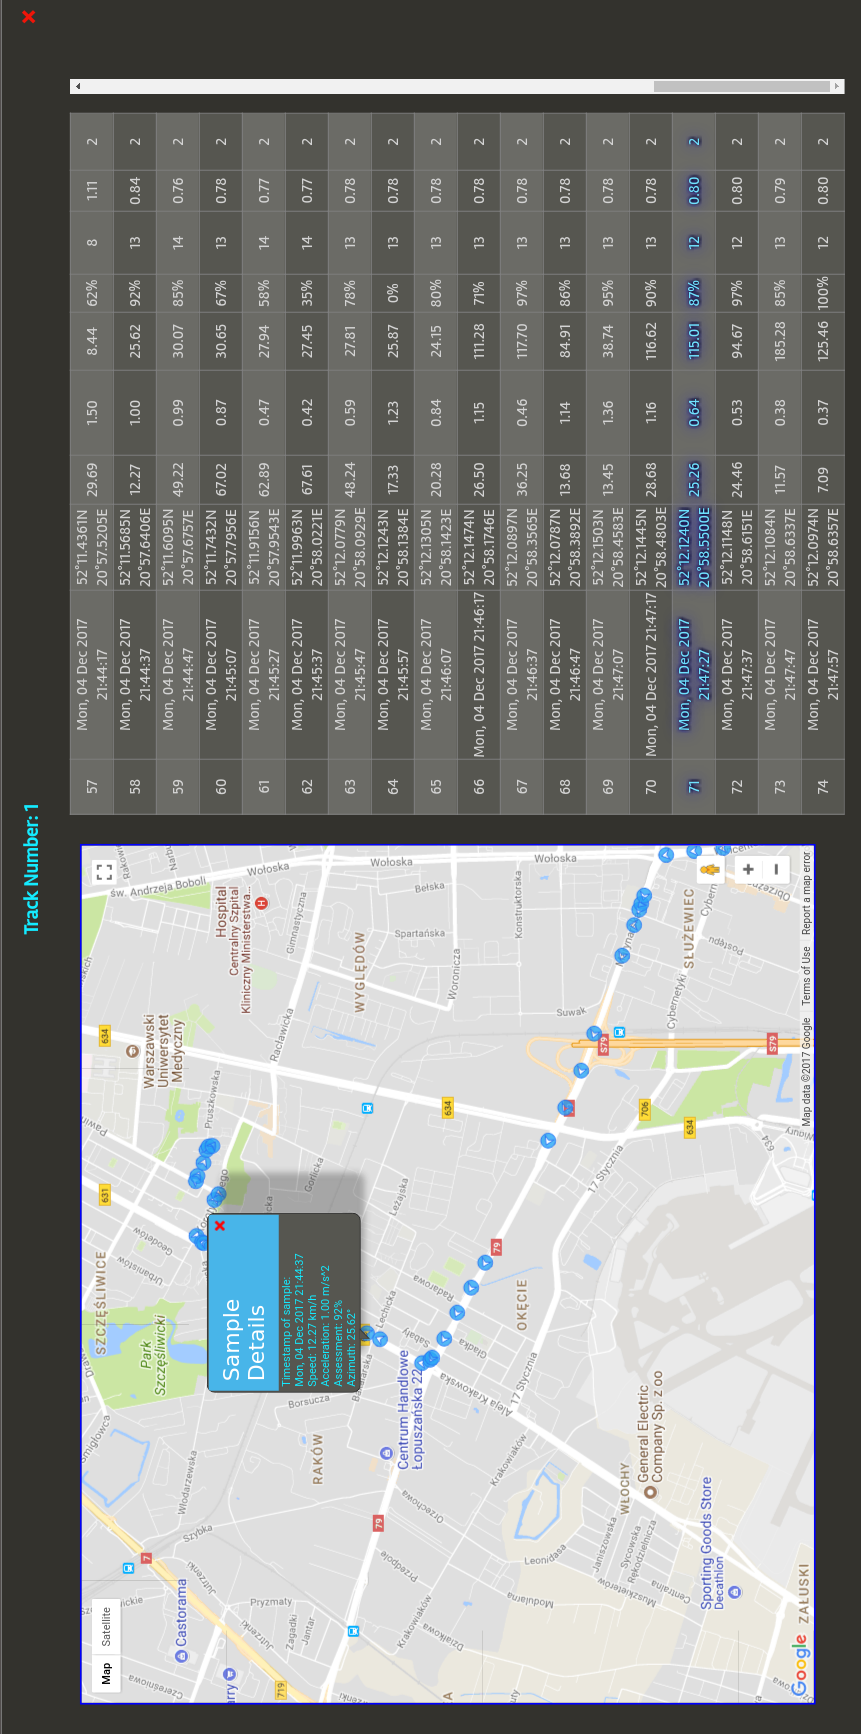
\includegraphics[height=19cm, width=13cm]{img/driving_analysis/test_track_part_4.png}
	\caption{Trasa próbna nr 1 - czwarta część trasy. Źródło: Opracowanie własne.}
	\label{fig:image_driving_analysis_alghoritm_track_1_part_4}
\end{figure}

Poniżej w celu zwiększenia przejrzystości danych, zestawiono je w tabeli dla przypadków łagodnej oraz dynamicznej jazdy.

\begin{table}[H]
\centering
\caption{Zestawienie próbek w przypadku jazdy łagodnej oraz agresywnej.\\ Źródło: Opracowanie własne.}
\label{table:table_driving_style_light}
\begin{tabular}{| P{4cm} | P{4cm} | P{4cm} | P{4cm} |}
\hline
\textbf{Czas pomiaru} &\textbf{Prędkość w momencie pomiaru $[km/h]$} & \textbf{Przyspieszenie średnie z okna pomiarowego $[m/{s^2}]$}	& \textbf{Ocena stylu jazdy} \\ \hline	
\multicolumn{4}{|c|}{\textbf{Jazda łagodna}}  \\ \hline	
04.12.2017 21:30:59	& 33.97	& 0.53 & 100\%	 \\ \hline	
04.12.2017 21:31:07	& 0.00	& 0.42 & 100\%	 \\ \hline	
04.12.2017 21:31:27	& 39.97	& 1.45 & 90\%	 \\ \hline	
04.12.2017 21:31:37 & 68.22	& 0.60 & 90\%	 \\ \hline	
04.12.2017 21:31:47	& 62.88	& 0.35 & 92\%	 \\ \hline	
04.12.2017 21:31:57	& 59.00	& 0.24 &	 93\%	 \\ \hline	
04.12.2017 21:32:17	& 16.84	& 1.14 & 92\%	 \\ \hline	
04.12.2017 21:32:27	& 48.93	& 0.97 & 74\%	 \\ \hline	
04.12.2017 21:32:37	& 62.78	& 0.25 &	 88\%	 \\ \hline	
04.12.2017 21:32:47	& 64.85	& 0.40 & 82\%	 \\ \hline	
04.12.2017 21:33:07	& 45.58	& 0.43 & 87\%	 \\ \hline	
04.12.2017 21:33:17	& 9.83	& 1.24 & 99\%	 \\ \hline	
04.12.2017 21:33:27 & 16.75	& 1.19 & 100\%	 \\ \hline	
\multicolumn{4}{|c|}{\textbf{Jazda dynamiczna}}  \\ \hline	
04.12.2017 21:36:07	& 40.16 & 2.18 & 49\%	 \\ \hline	
04.12.2017 21:36:17	& 68.77 	& 0.58 & 80\%	 \\ \hline	
04.12.2017 21:36:27	& 72.43	& 0.24 & 49\%	 \\ \hline	
04.12.2017 21:36:42  & 0.00	& 0.19 & 47\%	 \\ \hline	
04.12.2017 21:36:47 	& 68.02	& 0.24 & 71\%	 \\ \hline	
04.12.2017 21:36:57	& 57.57	& 0.38 &	 82\%	 \\ \hline	
04.12.2017 21:37:17	& 85.47	& 0.83 & 40\%	 \\ \hline	
04.12.2017 21:37:27	& 81.02	& 0.31 & 83\%	 \\ \hline	
04.12.2017 21:37:47	& 87.97	& 0.38 &	 49\%	 \\ \hline	
04.12.2017 21:38:07	& 88.36 & 0.54 & 53\%	 \\ \hline	
04.12.2017 21:38:17	& 81.36	& 0.66 & 42\%	 \\ \hline	
04.12.2017 21:38:37	& 0.22	& 0.85 & 100\%	 \\ \hline	
04.12.2017 21:38:57	& 38.20	& 1.55 & 86\%	 \\ \hline	
\end{tabular}
\end{table} 

Jak widać, wraz ze wzrostem dynamiki jazdy oceny zmalały, co dowodzi skuteczności algorytmu. Ponadto, można dostrzec iż oceny pomiędzy próbkami nie są ze sobą powiązane, dając możliwość do szybkiej korekcji stylu jazdy oraz nauki kierowania w sposób ekologiczny.
